\documentclass[oneside,a4paper,10pt]{report}

\usepackage{graphicx}
\usepackage{wrapfig}
\usepackage{lipsum}
\usepackage{color}
\usepackage{fancyhdr}
\usepackage{titlesec}
\usepackage[colorlinks=true,linkcolor=black]{hyperref}

%Setting up how paragraphs are formatted
%
\setlength{\parindent}{0mm}
\setlength{\itemsep}{0ex}
\setlength{\parskip}{2ex}
\setlength{\parsep}{2ex}
\setlength{\partopsep}{0ex}
\setlength{\topsep}{0ex}

%Swedish is supported once we add these packages
\usepackage[swedish]{babel}
\usepackage[T1]{fontenc}
\usepackage[utf8]{inputenc}

\bibliographystyle{IEEEtran}
\bibliography{referenser}

%\newcommand{\mychapter}[2]{
  %  \setcounter{chapter}{#1}
  %  \setcounter{section}{0}
 %   \chapter*{#2}
 %   \addcontentsline{toc}{chapter}{#2}
%}
\hypersetup{linktoc=all, urlcolor=black}

\title{
{\bf Inlämningsuppgift}\\
\vspace{0.2cm}
CCOM 17\\
\vspace{1cm}
Robert Nyquist\\Andreas Hagesjö\\
\vspace{1cm}
17 Oktober, 2013\\
}


\date{}
\begin{document}
\clearpage
\maketitle
\thispagestyle{empty}
\newpage


\newpage
\titleformat{\chapter}{\normalfont\huge\bfseries}{\thechapter}{1em}{}
\tableofcontents
\thispagestyle{empty}
\pagestyle{plain}
\newpage

%----------------------------------------------------------------------
\chapter{Answers}
\section{Question 1}
\subsection{a}
The hostname on one of our computers is Original-Hoogle with IP address 129.16.232.141
\subsection{b}
SInce this is a Linux computer the IP address can be found via the ifconfig command and hostname via the hostname command
\section{Question 2}
\subsection{a}
The packages cross the SUNET (Swedish University Computer Network)
\subsection{b}
You can find this route with the traceroute command.
Each router on the way to the destination returns an IMCP so that we are able to see all routers on the way and the time it takes to travel between them.
\section{Question 3}
\subsection{a}
A layered model makes it easier to study the different parts without caring about the other layers.
\subsection{b}
The internet model can be seen as either TCP/IP model or OSI model.
We choose the TCP/IP model which containes the following layers
\begin{itemize}
  \item Application
  \item Transport
  \item Internet
 \item Network access 
\end{itemize}

\subsubsection{Application}
Handles applications such as file transfer, mail and electronic login.
It displayes the data in a format that is easier for humans to use.

\subsubsection{Transport}
It provides an end-to-end(or host-to-host) connection using different protocols.
Example of protocols are TCP and UDP.

\subsubsection{Internet}
Transports the data from one host to another, and if needed trough different networks.
\subsubsection{Network access}
Provides physical connection between physical nodes.
It contains information about the hardware.
\subsection{c}
The phrase “a protocol operates between peer layers in two entities” means that each protocol talks with matching protocol on the other host without caring about the layers over or beneath the concerned layer.

\section{Question 4}
\subsection{a}
Telnet is a protocol for remote login with the following syntax: \\
telnet [host] [port]
\subsection{b}
telnet uses the telnet protocol, but uses TCP for sending packages.
The default port number is 23.

\section{Question 5}
\subsection{b}
www.kth.se is running on Apache/2.2.15 while www.sas.se runs on Microsoft-IIS/6.0.
Both servers respond with 200 OK which means taht our request has been accepted.
\newpage

\subsection{c}
\begin{figure}[h!]
  \caption{Request result from www.sas.se}
  \centering
    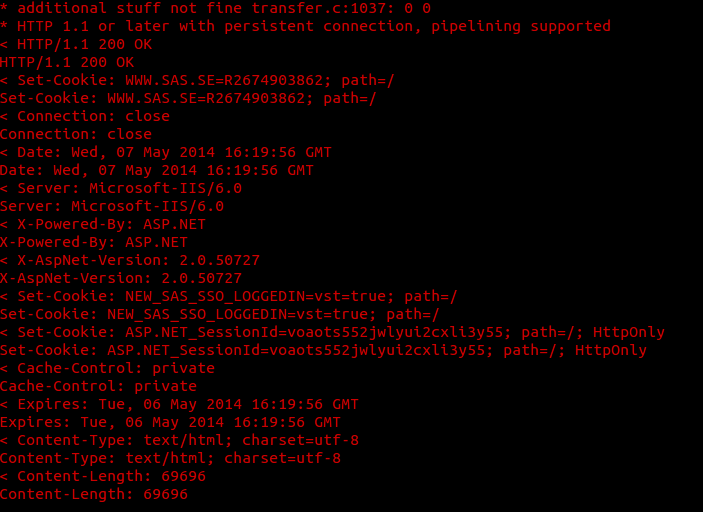
\includegraphics[scale=0.5]{sas}
\end{figure}



\begin{figure}[h!]
  \caption{Request result from www.kth.se}
  \centering
    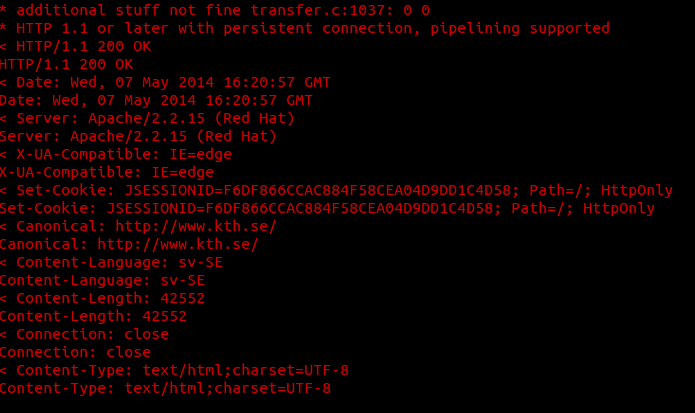
\includegraphics[scale=0.5]{kth.png}
\end{figure}

\newpage



\section{Question 6}
\subsection{a}
Examples of the types we found
\begin{itemize}
  \item Session management
  \item Personalization
  \item Tracking
\end{itemize}
\subsection{b}

\begin{itemize}
  \item The cookie containes
  \item The lifetime of the cookie
  \item A value - usually a randomly generated unique number
\end{itemize}

\section{Question 7}
\subsection{a}
Nslookup is used to determine which DNS-servers thats is used to translate an IP to a domain name.
Syntax: nslookup [host]
\subsection{b}
www.google.com got many IPs and it is used to devide the load on the server.

\section{Question 8}
\subsection{a}
IANA is responsible for the global coordination of the DNS Root, IP addressing, and other Internet protocol resources.
\subsection{b}
HTTP: Port 80 Telnet: Port 23 IMAP: Port 143 DNS: Port 53

\section{Question 9}
\subsection{a}
The timeout is calculated with three values, rtt from  current sample, an estimated rtt that is built on an average of a previous rtt sample and DevRTT which is a coefficient.
We want the timeout to be big enogh so that packages can arrive with some delay, but short enough so that we notice when a package is lost.
\subsection{b}
The timeout will increas. Since it's an unstable connection we want a higher timeout value to decreas the package loss and thus decreas the amount of packages being resent.





\end{document}
